\section{Versuchsaufbau}
In Abbildung \ref{abb:aufbau} ist die benötigte Versuchsapparatur schematisch dargestellt.
Das von einer Spektrallampe erzeugte Licht wird durch eine Sammellinse auf einen $D_1$-Filter fokussiert. Der $D_1$-Filter ist ein Interferenzfilter, der ein schmales Frequenzspektrum aus dem kontinuierlichem Spektrum herausselektiert. In diesem Versuchsaufbau ist die Frequenz so gewählt, dass nur die $D_1$-Linie des Rubidium-Spektrums ($\lambda=794,8\,\text{nm}$) durch den Filter gelassen wird.

Solch ein Filter ist in Abbildung \ref{abb:filter} zu sehen und besteht aus einem Dielektrikum der Dicke $d$ mit dem Brechungsindex $n$, welcher von einer reflektierenden Schicht umgeben ist. 
Diese Schicht ist für Licht halbdurchlässig und sorgt dafür, dass einfallendes Licht im Inneren des Filters mehrmals reflektiert wird.
Wellenlängen, welche der Bedingung
\begin{equation}
  j\lambda_j=2\cdot n\cdot d +\frac{\lambda}{2}~~~~j=2,3,...
\end{equation}
genügen, interferieren konstruktiv. 
Im idealen Fall von vielen Reflexionen wird Licht mit anderer Wellenlänge durch destruktive Interferenz ausgelöscht.
Um Licht einer bestimmten Wellenlänge $\lambda_k$ herauszufiltern, wird der Interferenzfilter mit Farbfiltern kombiniert, die andere Wellenlängen auslöschen sollen. 
Da die reflektierende Schicht nicht alle Strahlen reflektiert, sind nur endliche viele Reflexionen möglich.
Daher werden in der Umgebung von $\lambda_k$ nicht alle Wellenlängen ausgelöscht. 
Umso höher der Reflexionskoeffizient der Schicht, desto schmaler ist das selektierte Frequenzspektrum. (aus unserem Faraday-Effekt-Protokoll...)

Dann wird das Licht der gewünschten Spektrallinie durch einen Linearpolarisator linear polarisiert und dann durch ein $\lambda/4$-Plättchen zirkular polarisiert.

Ein $\lambda/4$-Plättchen ist eine besondere Verzögerungsplatte.
Eine Verzögerungsplatte besteht aus anisotropem Material, wodurch  es zwei zueinander senkrechte Achsen gibt, in dessen Richtungen sich Licht mit den Geschwindigkeiten $v_\text{langsam}=\frac{c}{n_\text{langsam}}$ und $v_\text{schnell}=\frac{c}{n_\text{schnell}}$ ausbreitet. $c$ ist dabei die Lichtgeschwindigkeit im Vakuum.
In einer Verzögerungsplatte der Dicke $d$ wird so der Phasenunterschied um 
\begin{equation*}
  \Delta \phi=\frac{2\pi}{\lambda}\cdot d \cdot (n_\text{langsam}-n_\text{schnell})
\end{equation*}
verschoben.
Da ein $\lambda/4$-Plättchen aus linar polarisiertem Licht zirkular polarisiertes Licht erzeugen soll, muss die Dicke des $\lambda/4$-Plättchens so gewählt werden, dass die Phasenverschiebung $\Delta \phi$ beim Durchlaufen des Lichtes durch die Platte genau $\pi/2$ beträgt. Die schematische Funktionsweise des $\lambda/4$-Plättchens ist in Abbildung \ref{abb:l4} zu sehen.

Das nun zirkular polarisierte Licht fällt jetzt auf eine Dampfzelle, dessen Temperatur sich mit einer Heizung steuern lässt, um den idealen Rubidium-Dampfdruck zu erzeugen.
Durch eine Modulationsfeldspule (auch Sweep-Spule genannt; $R=16,39\,\text{cm}$, $N=11$) und eine Horizontalfeldspule ($R=15,79\,\text{cm}$, $N=154$) lassen sich zwei horizontale Magnetfelder um die Dampfzelle erzeugen. Zudem wird durch eine Vertikalfeldspule ($R=11,735\,\text{cm}$, $N=20$) ein vertikales Feld erzeugt. Alle drei Feldstärken lassen sich durch die Feldstromversorgung getrennt voneinander einstellen. Die Ströme lassen sich durch Potentiometer ziemlich genau variieren. Der Strom der Vertikal-Spulen wird pro Umdrehung des Potentiometers um $0,1\,\text{A}$ verändert und der maximale Spulenstrom beträgt für diese Spulen $I_\text{max}=1\,\text{A}$.  Der Strom der Horizontal-Spule wird pro Umdrehung des Potentiometers um $0,3\,\text{A}$ verändert und der maximale Spulenstrom beträgt  $I_\text{max}=3\,\text{A}$.
Die Sweep-Spule lässt sich zudem durch einen Kontrollgerät langsam variieren. An diesem Gerät werden ein Startwert, eine Amplitude und die Durchlaufdauer eingestellt.

Wenn das Licht wieder aus der Dampfzelle tritt, wird durch eine Sammellinse auf einen Lichtdetektor abgebildet. In diesem Aufbau wird ein Si-Photoelement verwendet, dessen Signal durch einen Linearverstärker verstärkt und dann auf den Y-Eingang eines Oszilloskops gegeben wird. Durch diesen können Schwankungen der Lichtintensität gemessen werden.
 
<<<<<<< HEAD
 \begin{figure}[H]
	\centering
	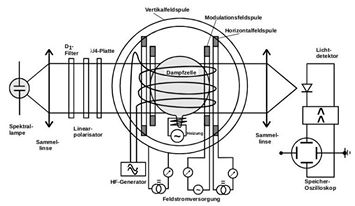
\includegraphics[width=12cm]{aufbau.jpg}
=======
 \begin{figure}[H]
	\centering
	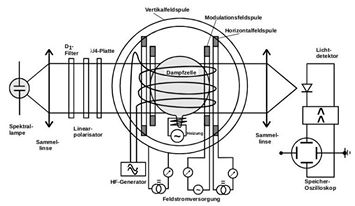
\includegraphics[width=12cm]{aufbau.jpg}
>>>>>>> c40044fcbae27fa508ec0d1cb0974b0c9018ab0a
	\caption{schematisch dargestellte Versuchsapparatur \cite{V21}}
	\label{abb:aufbau}
\end{figure}

\begin{figure}
    \centering
    \begin{subfigure}[c]{0.19\textwidth}
        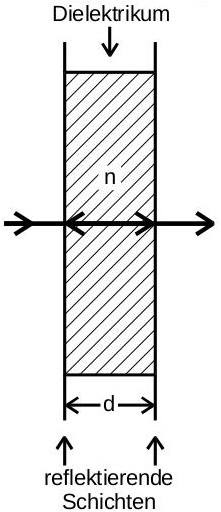
\includegraphics[width=\textwidth]{filter.jpg}
        \caption{Interferenzfilter \cite{V46}}
        \label{abb:filter}
    \end{subfigure}
      \begin{subfigure}[c]{0.8\textwidth}
        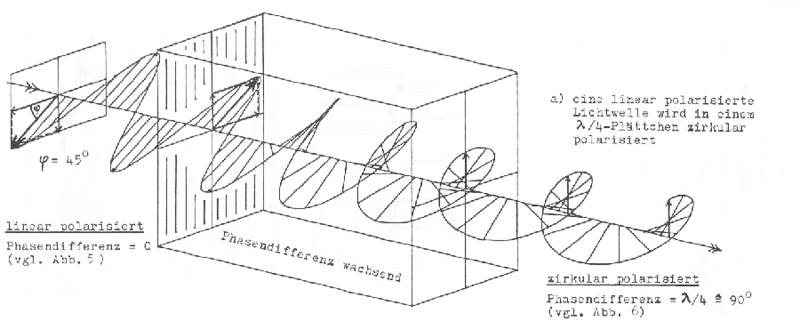
\includegraphics[width=\textwidth]{l42.png}
        \caption{Funktionsweise des $\lambda/4$-Plättchens \cite{wiki}}
        \label{abb:l4}
    \end{subfigure}
    \caption{verwendete Instrumente}
\end{figure}
